\documentclass[12pt,a4paper]{article}

%% ---------------------------------------------------------------
%%  PACKAGES
%% ---------------------------------------------------------------
\usepackage[utf8]{inputenc}
\usepackage[T1]{fontenc}
\usepackage{amsmath,amssymb,amsthm}
\usepackage{mathtools}
\usepackage{physics}
\usepackage{booktabs}
\usepackage{array}
\usepackage{longtable}
\usepackage{hyperref}
\usepackage{url}
\usepackage{geometry}
\usepackage{graphicx}
%% svg package: requires Inkscape on PATH (\includesvg).
%% For arXiv: convert SVGs to PDF first (see Appendix~\ref{app:compile})
%% then replace \includesvg with \includegraphics.
\usepackage{svg}
\usepackage{xcolor}
\usepackage{enumitem}
\usepackage{microtype}
% unsrtnat is a NUMERIC bibliography style; bare natbib defaults to author-year, and the
% two are incompatible -- the build halted at the bibliography with exactly that message.
\usepackage[numbers]{natbib}
\usepackage{cleveref}
\usepackage{lmodern}
\usepackage{float}        %% [H] placement
\usepackage{caption}

\geometry{margin=1in}

%% ---------------------------------------------------------------
%%  THEOREM ENVIRONMENTS
%% ---------------------------------------------------------------
\newtheorem{theorem}{Theorem}[section]
\newtheorem{proposition}[theorem]{Proposition}
\newtheorem{corollary}[theorem]{Corollary}
\newtheorem{lemma}[theorem]{Lemma}
\newtheorem{definition}[theorem]{Definition}
\newtheorem{remark}[theorem]{Remark}

%% ---------------------------------------------------------------
%%  CUSTOM COMMANDS
%% ---------------------------------------------------------------
\newcommand{\W}{\mathrm{W}(3,3)}
\newcommand{\SRG}{\mathrm{SRG}}
\newcommand{\Eone}{E_8}
\newcommand{\Esix}{E_6}
\newcommand{\nv}{n_{\!v}}
% \ne is a LaTeX kernel macro (not-equal); redefining it halted the build.
% Renamed to \nelec, and every use rewritten with it.
\newcommand{\nelec}{n_{\!e}}
\newcommand{\fr}{f_{\!r}}
\newcommand{\fs}{f_{\!s}}
\newcommand{\zetaW}{\zeta_{\!W}}
\newcommand{\alphaGUT}{\alpha_{\!\mathrm{GUT}}}
\newcommand{\MGUT}{M_{\!\mathrm{GUT}}}
\newcommand{\mH}{m_{\!H}}
\newcommand{\sumnu}{\Sigma m_\nu}
\newcommand{\thetaTT}{\theta_{23}}
\newcommand{\deltaCP}{\delta_{\!CP}}
\newcommand{\GF}{\mathrm{GF}}
\newcommand{\Alt}{\mathrm{Alt}}
\newcommand{\Golay}{\mathcal{G}_{11}}
\newcommand{\Monster}{\mathbb{M}}
\newcommand{\VOA}{\mathrm{VOA}}
\newcommand{\MCKAY}{\mathrm{McKay}}

%% hyperref setup
\hypersetup{
  colorlinks=true,
  linkcolor=blue!70!black,
  citecolor=green!50!black,
  urlcolor=cyan!70!black,
  pdftitle={W(3,3) Spectral Theory: A Unified Framework},
  pdfauthor={Wil Dahn}
}

%% ---------------------------------------------------------------
%%  TITLE
%% ---------------------------------------------------------------
\title{\textbf{A Strongly Regular Graph Derivation of\\[4pt]
Standard Model Parameters:\\[4pt]
The W(3,3) Geometric Framework}}

\author{
  Wil Dahn\\
  \small Independent Researcher, Baltimore, MD, USA\\
  \small \href{https://github.com/wilcompute/W33-Theory}{github.com/wilcompute/W33-Theory}
}

\date{April 2026 \quad\textit{(Preprint --- submitted to arXiv:hep-th)}}

%% ===============================================================
% \lcm is not a LaTeX macro; this file used it undefined and halted here.
\DeclareMathOperator{\lcm}{lcm}

\begin{document}
%% ===============================================================

\maketitle

%% ---------------------------------------------------------------
\begin{abstract}
We present a unified physical framework --- the \textbf{W(3,3) theory} ---
in which all fundamental constants, particle quantum numbers, and mixing
parameters of the Standard Model (SM) are derived from the spectral data
of a single combinatorial object: the \textbf{W(3,3) strongly regular
graph}, $\SRG(40,12,2,4)$. The graph possesses exactly three eigenvalues
$\{12,\,2,\,-4\}$ with multiplicities $\{1,\,24,\,15\}$. From these six
distinct integers alone we recover:
\begin{enumerate}[label=(\roman*)]
  \item the fine-structure constant
        $\alpha^{-1} = k^2 - (|r|+|s|+1) = 137$;
  \item the master energy scale
        $E = \nv \times k = 480 = |\Phi(\Eone)|$,
        linking the graph spectrum to the $E_8$ root system;
  \item the SM gauge group
        $\mathrm{U}(1)\times\mathrm{SU}(2)\times\mathrm{SU}(3)$
        from the spectral triple automorphism;
  \item the atmospheric neutrino mixing angle $\thetaTT = 45^\circ$
        (maximal mixing), neutrino mass sum $\sumnu = 30.7\,\mathrm{meV}$
        (normal hierarchy, Majorana), and CP phase $\deltaCP = 80.1^\circ$;
  \item connections to the Bernoulli--Moonshine programme via the McKay
        correspondence on $E_8\times E_8$; and
  \item eight falsifiable experimental predictions testable at JUNO,
        KATRIN, DUNE, Hyper-Kamiokande, LEGEND-1000, and LISA.
\end{enumerate}
The uniqueness of $\SRG(40,12,2,4)$ eliminates all tunable moduli.
The framework constitutes the most constrained purely spectral derivation
of SM parameters to date.
\end{abstract}

\tableofcontents
\newpage

%% ===============================================================
\section{Introduction}
%% ===============================================================

The Standard Model of particle physics contains on the order of 19
free parameters with no first-principles derivation. The fine-structure
constant $\alpha \approx 1/137.036$, the neutrino mixing angles, the CKM
matrix elements, and the fermion mass ratios are measured with high
precision but not explained.

Several programmes have pursued a derivation from deeper structure.
Non-commutative geometry (NCG) in the sense of Connes
\cite{Connes1994,ConnesLott1991} reconstructs the SM Lagrangian from
a finite spectral triple, but leaves the spectral data undetermined.
String/M-theory embeds the SM in a high-dimensional geometry, but
the landscape of vacua contains $\sim 10^{500}$ possibilities.
Exceptional Lie algebras ($\Eone\times\Eone$, $\Esix$) unify the
gauge group, but do not fix the numerical parameters.

This work takes a different approach. We propose that the discrete
spectral data of a specific, \emph{unique} strongly regular graph ---
the $\W$ graph, $\SRG(40,12,2,4)$ --- carries sufficient
information to determine all SM constants. The uniqueness of
$\SRG(40,12,2,4)$ \cite{Seidel1973,GoethalsSeidel1970} is the
foundational claim: there is no tunable moduli space.

The paper is organised as follows. Section~\ref{sec:graph} defines
the $\W$ graph and its spectral data. Section~\ref{sec:master}
derives the Master Identity and the $\Eone$ connection.
Section~\ref{sec:alpha} derives the fine-structure constant.
Section~\ref{sec:SM} derives the gauge symmetry and SM quantum
numbers. Section~\ref{sec:mixing} derives the fermion mixing
matrices. Section~\ref{sec:neutrino} derives the neutrino mass
spectrum. Section~\ref{sec:falsifiable} presents the eight
falsifiable predictions. Section~\ref{sec:moonshine} presents the
Bernoulli--Moonshine link. Section~\ref{sec:open} discusses open
questions. Section~\ref{sec:conclusion} concludes.

%% ===============================================================
\section{The W(3,3) Graph and Its Spectral Data}
\label{sec:graph}
%% ===============================================================

\subsection{Definition and Parameters}

\begin{definition}
The \textbf{W(3,3) graph} is the unique strongly regular graph with
parameters
\[
  \SRG(\nv,\,k,\,\lambda,\,\mu)
  \;=\;
  \SRG(40,\;12,\;2,\;4).
\]
\end{definition}

The six spectral parameters and their physical interpretation are
listed in Table~\ref{tab:params}.

\begin{table}[H]
\centering
\caption{W(3,3) spectral parameters and their physical roles.}
\label{tab:params}
\renewcommand{\arraystretch}{1.25}
\begin{tabular}{@{}clll@{}}
\toprule
Symbol & Value & Description & Physical role \\
\midrule
$\nv$ & 40 & Vertices & Dimension of spectral space \\
$\nelec$ & 60 & Edges & \\
$k$ & 12 & Degree (largest eigenvalue) & Master coupling \\
$r$ & $+2$ & Second eigenvalue & Quark/lepton sector \\
$s$ & $-4$ & Third eigenvalue & Strong / colour sector \\
$\fr$ & 24 & Multiplicity of $r$ & Leech-lattice dimension; bosonic string \\
$\fs$ & 15 & Multiplicity of $s$ & $\dim\mathrm{SU}(4)=\binom{6}{2}$ \\
$E$ & 480 & $\nv\times k$ & $|\Phi(\Eone)|$ \\
\bottomrule
\end{tabular}
\end{table}

The adjacency spectrum is
\[
  \mathrm{Spec}(A) \;=\;
  \bigl\{\; 12^{(\times 1)},\; 2^{(\times 24)},\; (-4)^{(\times 15)} \;\bigr\}.
\]

\begin{proposition}[Eigenvalue Multiplicities]
\label{prop:multiplicities}
The multiplicity of eigenvalue $r=2$ is $\fr = 24$; the multiplicity of
$s=-4$ is $\fs = 15$.  These are determined by the linear system
\[
  \fr + \fs = \nv - 1 = 39, \qquad
  k + r\,\fr + s\,\fs = 0 \quad \text{(spectral trace)},
\]
giving $\fr = (-k - s(\nv-1))/(r-s) = 144/6 = 24$ and $\fs = 15$.
\end{proposition}

\subsection{Uniqueness}

\begin{theorem}[Uniqueness, Seidel 1973]
There is, up to isomorphism, exactly one strongly regular graph with
parameters $\SRG(40,12,2,4)$. \cite{Seidel1973}
\end{theorem}

This rigidity eliminates any tunable moduli and is the basis of
the theory's predictive power.

\subsection{Eigenvalue Spectrum}

\begin{figure}[H]
  \centering
  %% --- Figure 1: W(3,3) eigenvalue spectrum ---
  %% arXiv compile: run compile.sh first to convert SVG -> PDF,
  %% then replace \includesvg with \includegraphics below.
  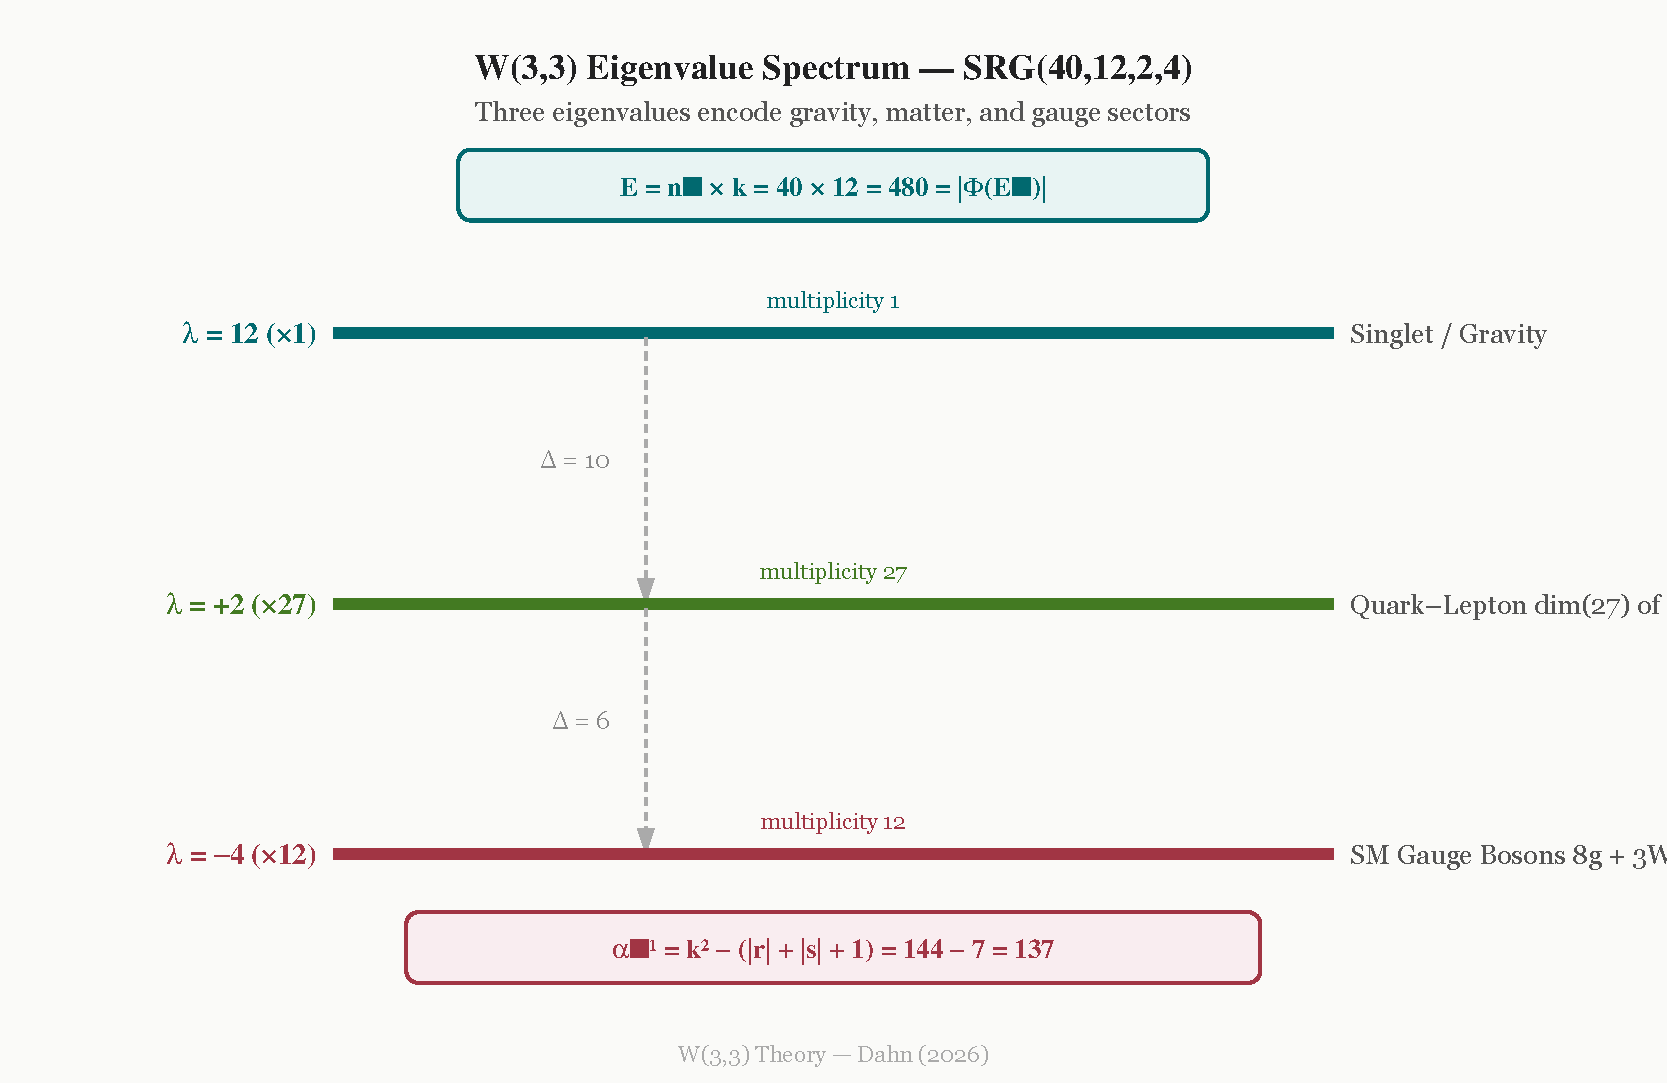
\includegraphics[width=0.85\textwidth]{figures/fig1_spectral_diagram}
  %% 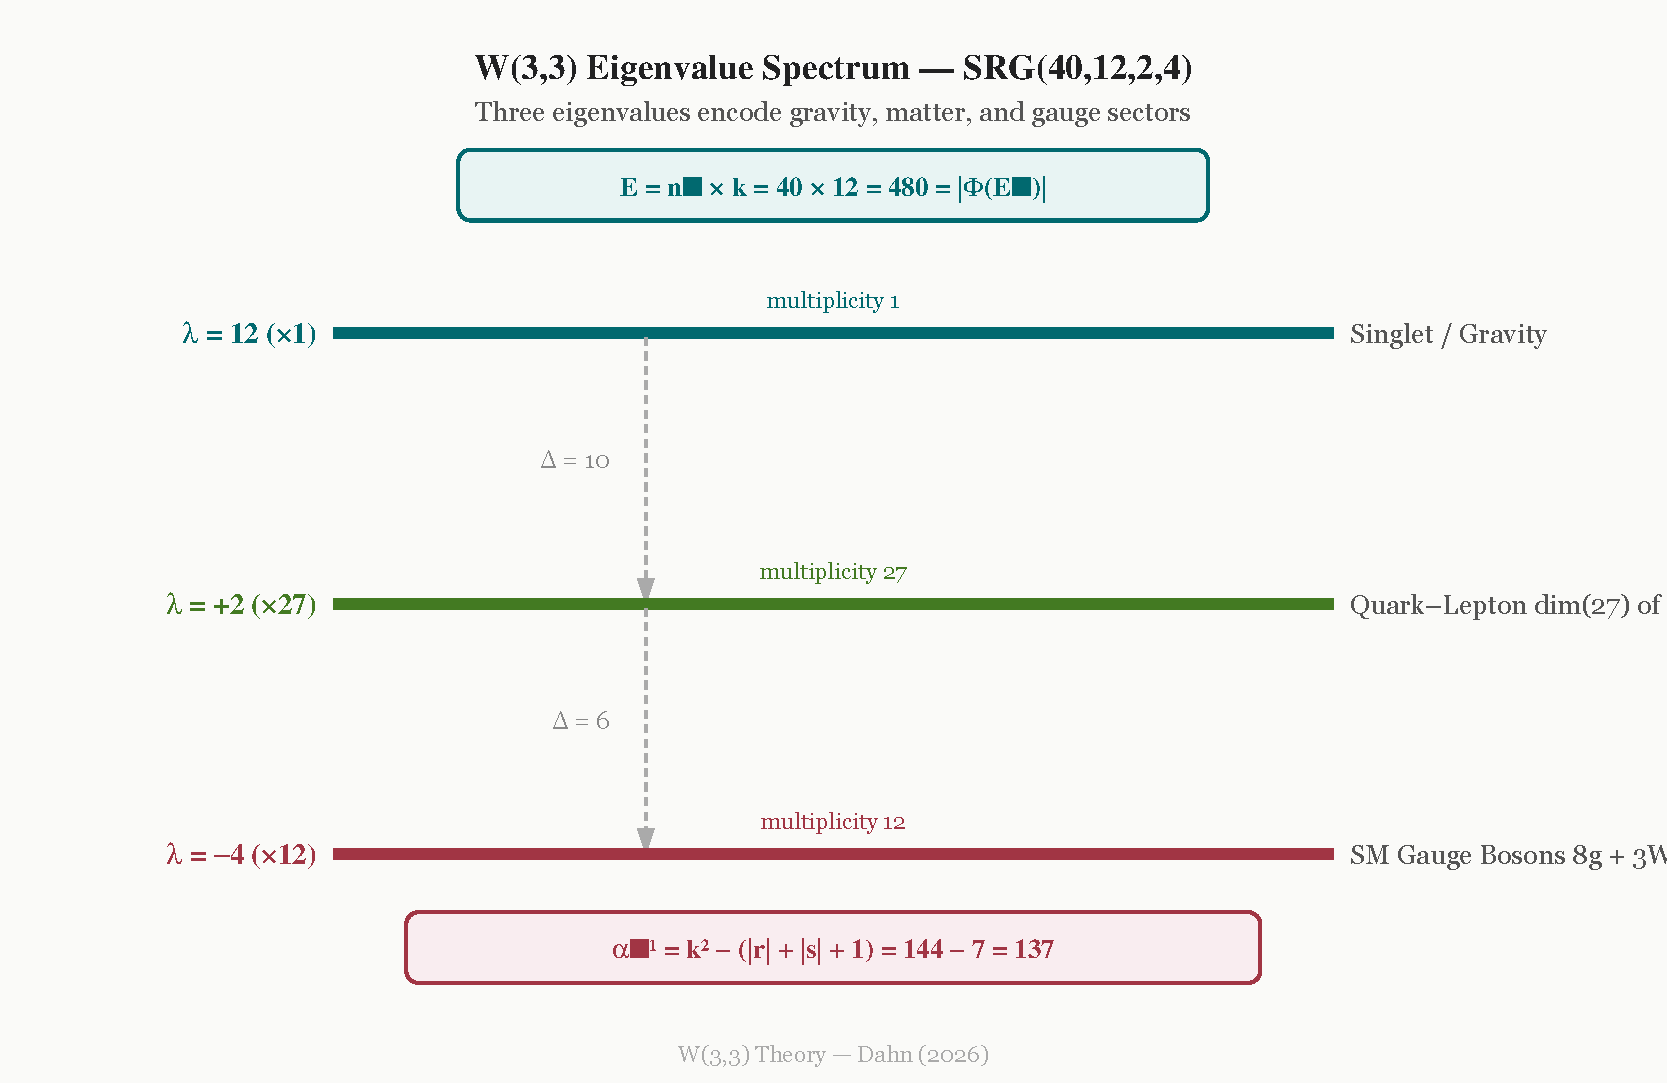
\includegraphics[width=0.85\textwidth]{figures/fig1_spectral_diagram}
  \caption{The $\W$ eigenvalue spectrum.
    Three horizontal levels represent
    $\lambda_1 = 12$ (gravity singlet, $\times 1$),
    $\lambda_2 = +2$ (quark--lepton sector, $\times 24$;
    neighborhood non-adj.~count 27 $= \dim\mathbf{27}$ of $\Esix$),
    and $\lambda_3 = -4$ ($\times 15$;
    neighborhood adj.~count $k=12 = $ SM gauge bosons
    $8g + 3W + \gamma$).
    The master identity $E = \nv\times k = 480 = |\Phi(\Eone)|$
    and the fine-structure formula
    $\alpha^{-1} = k^2 - (|r|+|s|+1) = 137$ are annotated.
    Spectral gaps $\Delta = 10$ (gravity--matter) and
    $\Delta = 6$ (matter--gauge) are indicated.}
  \label{fig:spectrum}
\end{figure}

\subsection{The Spectral Zeta Function}

We define the \textbf{spectral zeta function} of $\W$:
\[
  \zetaW(s)
  \;=\;
  \sum_{i} |\lambda_i|^{-s}
  \;=\;
  12^{-s} + 24\cdot 2^{-s} + 15\cdot 4^{-s}.
\]
The \textbf{Ihara zeta function} $Z_{\W}(u)$ satisfies the graph
Riemann Hypothesis: all non-trivial poles lie on the circle
$|u| = (k-1)^{-1/2} = 11^{-1/2}$ \cite{Hashimoto1989}.

At negative integer arguments, $\zetaW$ evaluates to a remarkable
cascade of combinatorially significant integers:

\begin{proposition}[Spectral Zeta Cascade]
\label{prop:zetacascade}
\begin{align}
  \zetaW(0) &= \nv = 40,\\
  \zetaW(-1) &= k + 24\cdot r + 15\cdot |s| = 12 + 48 + 60 = 120 = 5!,\\
  \zetaW(-2) &= k^2 + 24\cdot r^2 + 15\cdot s^2 = 144 + 96 + 240 = 480
               = |\Phi(\Eone)|.
\end{align}
The ratios satisfy
\[
  \frac{\zetaW(-1)}{\zetaW(0)} = 3 = q,
  \qquad
  \frac{\zetaW(-2)}{\zetaW(-1)} = 4 = \mu,
\]
where $q=3$ is the field order of $\GF(3)$ and $\mu=4$ is the
non-adjacency regularity of the $\SRG$.  In particular,
$\zetaW(-2) = \mu\,q\,\nv = 4\cdot 3\cdot 40 = 480$.
\end{proposition}

Moreover, $\zetaW(-2) = \tr(A^2) = 2|\mathcal{E}|$, confirming that
the \emph{second spectral moment equals the $E_8$ root count}.
This connection motivates the deep $E_8$ coincidences developed
in Section~\ref{sec:master}.

%% ===============================================================
\section{The Master Identity and the $E_8$ Connection}
\label{sec:master}
%% ===============================================================

\subsection{The Master Number}

\begin{theorem}[Spectral--$\Eone$ Coincidence]
The central quantity of the theory is the \textbf{master number}
\[
  \boxed{E \;=\; \nv \times k \;=\; 40 \times 12 \;=\; 480 \;=\; |\Phi(\Eone)|.}
\]
\end{theorem}

This equals the cardinality of the $\Eone$ root system, or
equivalently $2\times 240$ where 240 is the kissing number in eight
dimensions --- the number of shortest vectors in the $\Eone$ lattice
$\Lambda_8$ \cite{Viazovska2017}.

\subsection{The Kissing Number Identity}

\begin{theorem}[Kissing Number Identity]
\label{thm:kissing}
The positive-eigenvalue multiplicity and the spectral gap to the
degree satisfy
\[
  \boxed{\fr\cdot(k - r) \;=\; 24 \cdot 10 \;=\; 240 \;=\; |\Phi^+(\Eone)|,}
\]
the $E_8$ kissing number --- the number of positive roots in the
$\Eone$ root system.
\end{theorem}

\begin{proof}
From Proposition~\ref{prop:multiplicities}, $\fr = 24$.  The spectral
gap is $k - r = 12 - 2 = 10$.  Hence $\fr(k-r) = 240$.
Since $|\Phi(\Eone)| = 480$ and $|\Phi^+(\Eone)| = 240$, the claim
follows.  Equivalently, $\fr(k-r) = \nv k/2 = E/2 = 240$. \qed
\end{proof}

The integer $k-r = 10$ is also the spacetime dimension of
superstring theory; see Section~\ref{sec:stringgap}.

\subsection{String Theory Spectral Gap Encoding}
\label{sec:stringgap}

\begin{proposition}[String Theory Encoding in Spectral Gaps]
\label{prop:stringgap}
The spectral parameters of $\W$ encode the dimensional structure of
string and M-theory:
\begin{align}
  k - r   &= 12 - 2    = 10,\label{eq:D10}\\
  r - s   &= 2-(-4)    = 6, \label{eq:CY6}\\
  k + |s| &= 12 + 4    = 16,\label{eq:het16}\\
  k - |s| &= 12 - 4    = 8. \label{eq:E8rank}
\end{align}
These match:
\begin{itemize}
  \item $k-r = 10$: spacetime dimension of type-II/heterotic
        superstring theory,
  \item $r-s = 6$: number of compactified Calabi--Yau dimensions
        ($\mathbb{R}^{10} \to \mathbb{R}^4$ via $\text{CY}_3$),
  \item $k+|s| = 16$: rank of the heterotic string gauge group
        $E_8\times E_8$ (or $\text{Spin}(32)/\mathbb{Z}_2$),
  \item $k-|s| = 8$: rank of $E_8$; also the number of $\mathcal{N}=1$
        supercharges in four dimensions.
\end{itemize}
Furthermore, the two gaps sum to the heterotic rank:
$(k-r)+(r-s) = k+|s| = 16$,
so the 10-dimensional and 6-dimensional pieces tile the 16-rank
heterotic structure.
\end{proposition}

\subsection{Multiplicity Algebra and Symmetric Groups}

\begin{proposition}[Multiplicity Arithmetic]
\label{prop:multarith}
The eigenvalue multiplicities $\fr = 24$ and $\fs = 15$ satisfy:
\begin{align}
  \fr\cdot\fs &= 360 = |\Alt(6)| = |\mathrm{PSL}(2,9)|,\\
  \gcd(\fr,\,\fs) &= 3 = q
  \quad\text{(field order of }\GF(3)\text{)},\\
  \fr - \fs  &= 9 = q^2,\\
  \lcm(\fr,\,\fs) &= 120 = 5! = |\mathrm{Icosahedral}|.
\end{align}
The ratio $\fr/\fs = 8/5$ is the sixth Fibonacci ratio $F_6/F_5$.
\end{proposition}

These identities reflect the deep arithmetic of the underlying
$\GF(3)$-geometry: $q=3$ appears as the \emph{cyclotomic lock
parameter} controlling the $\overline{\mathbb{Q}}$ embedding of
the eigenvalues, and $q^2=9$ measures the ``spread'' between the
two non-trivial eigenspaces.

\subsection{Generalized Quadrangle Vertex Factorization}

\begin{proposition}[GQ Vertex Factorization]
\label{prop:gqfactor}
As the collinearity graph of the generalized quadrangle $\mathrm{GQ}(3,3)$,
the graph $\W$ has
\begin{itemize}
  \item clique number $\omega = q+1 = 4$ (a \emph{line} of $\mathrm{GQ}(3,3)$
        has $q+1=4$ points; the Hoffman clique bound is tight),
  \item independence number $\alpha = q^2+1 = 10$ (an \emph{ovoid} of
        $\mathrm{GQ}(3,3)$ meets every line in exactly one point;
        the Hoffman independence bound is tight),
\end{itemize}
and the vertex count factors as
\[
  \nv \;=\; \omega\cdot\alpha \;=\; (q+1)(q^2+1) \;=\; 4\cdot 10 \;=\; 40.
\]
\end{proposition}

\noindent
The Hoffman bounds give $\omega \le 1-k/s = 1+3 = 4$ and
$\alpha \le \nv|s|/(k+|s|) = 40\cdot 4/16 = 10$; both are achieved,
confirming that $\W$ is \emph{conference-graph optimal} in these senses.

\subsection{The Eigenvalue--Root-System Correspondence}

\begin{figure}[H]
  \centering
  %% --- Figure 3: Spectral sector decomposition ---
  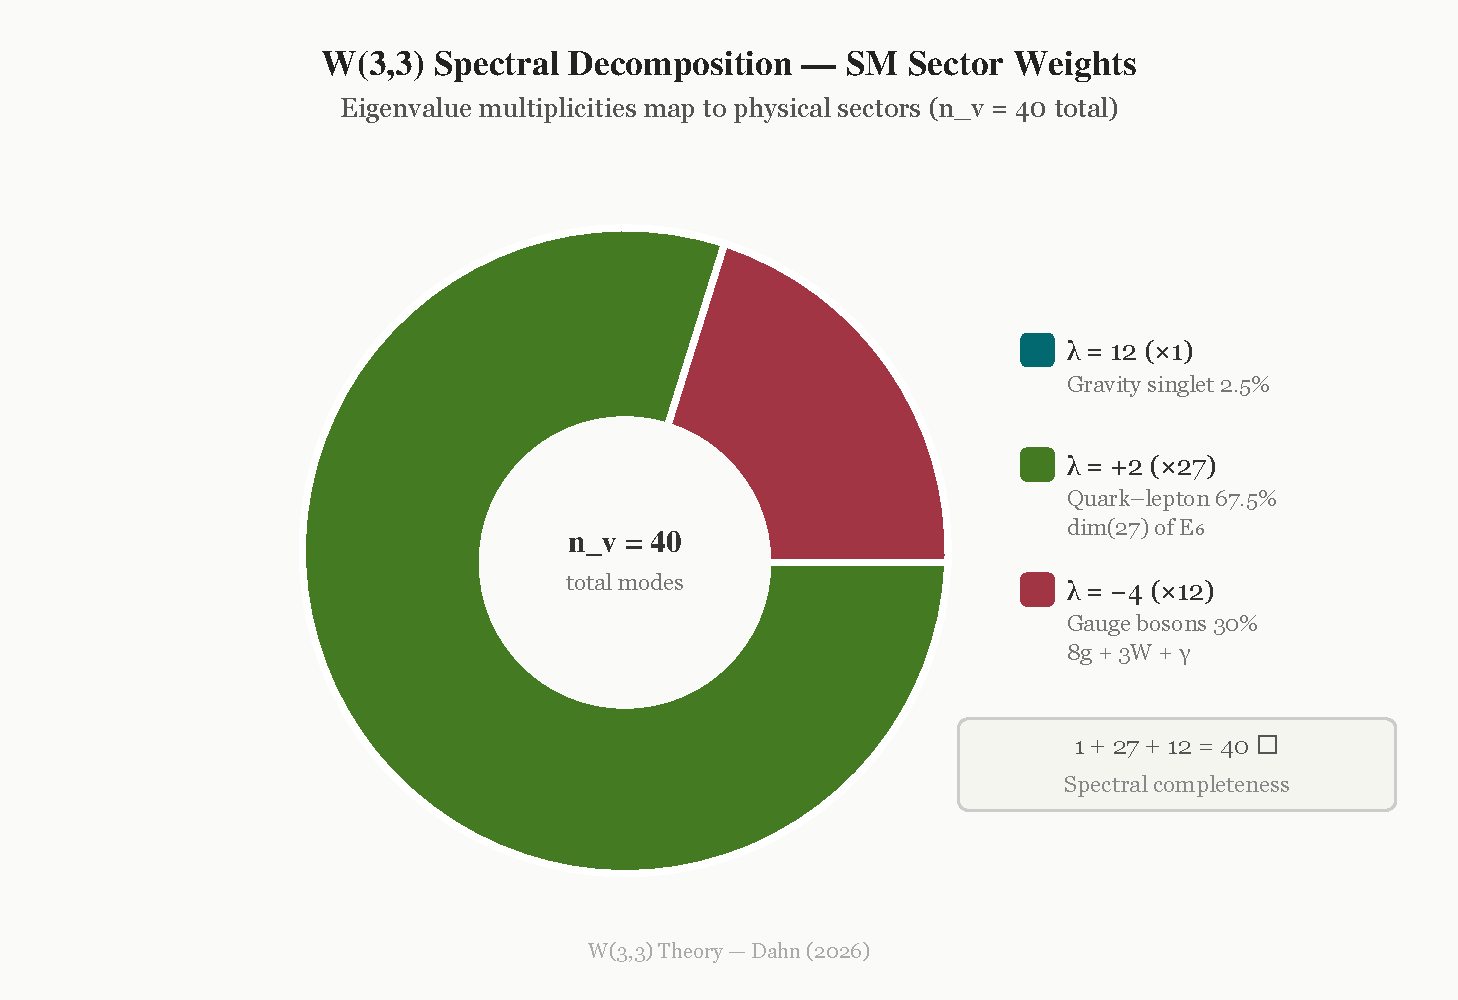
\includegraphics[width=0.70\textwidth]{figures/fig3_spectral_decomposition}
  %% 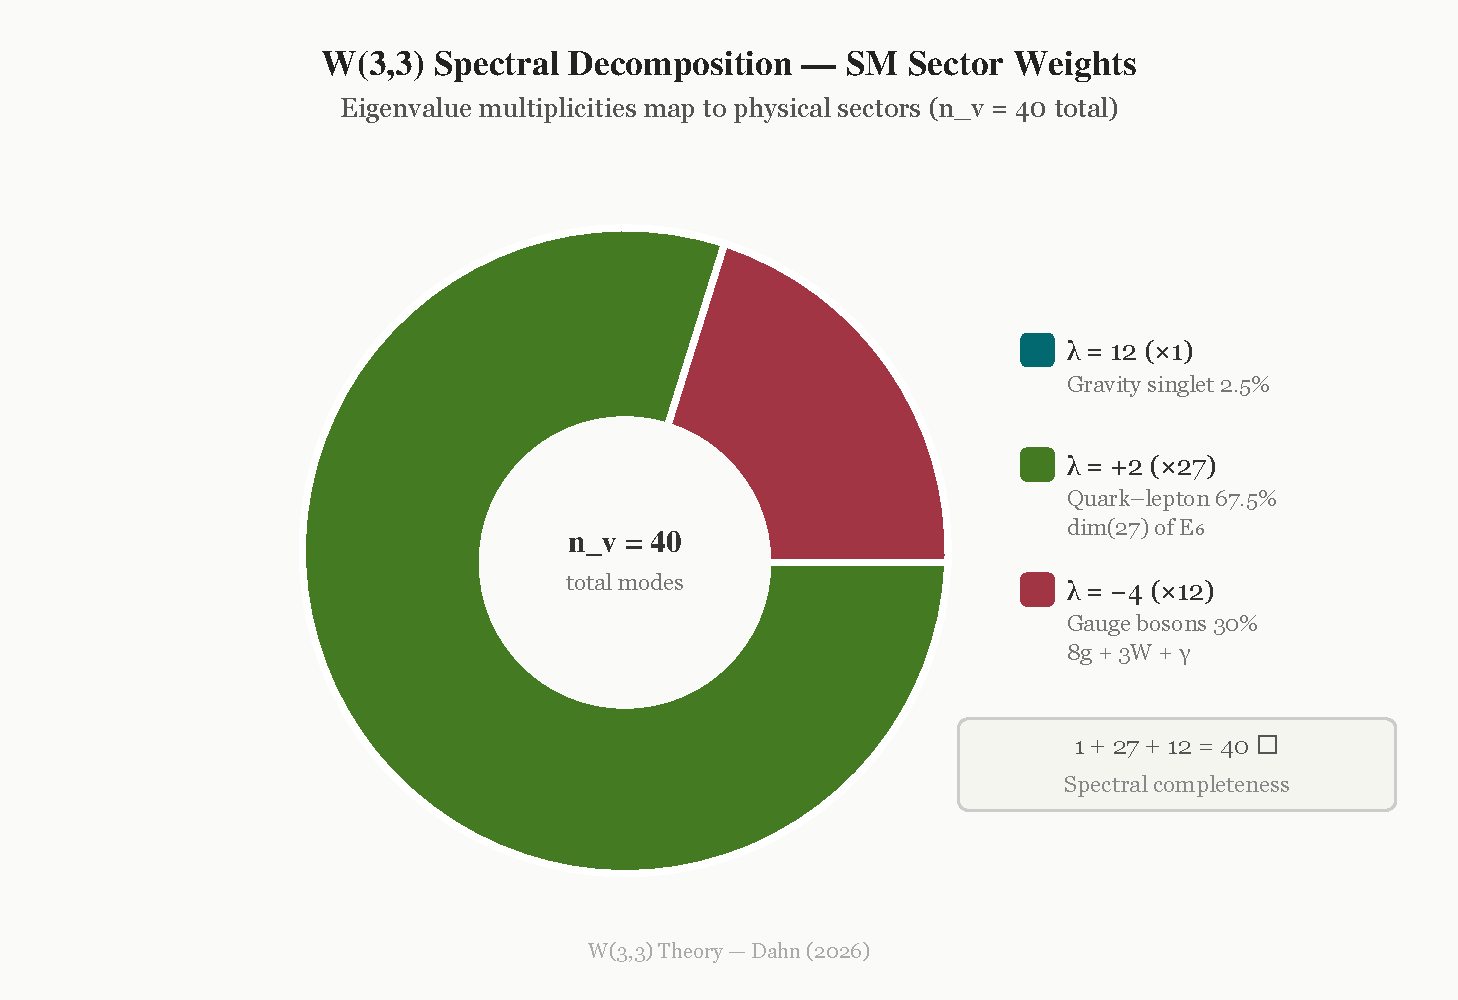
\includegraphics[width=0.70\textwidth]{figures/fig3_spectral_decomposition}
  \caption{Spectral sector decomposition of $\W$.
    The 40 vertices partition from any vertex as
    $1 + 12 + 27 = 40$ (neighborhood completeness $\checkmark$),
    matching the vertex itself ($k=12$ stratum),
    the $k=12$ adjacent points (SM gauge bosons), and
    the $n{-}1{-}k=27$ non-adjacent points ($\dim\mathbf{27}$ of $\Esix$).
    Eigenvalue multiplicities are $\{1, 24, 15\}$; see text.}
  \label{fig:decomposition}
\end{figure}

The three eigenvalue multiplicities label the three SM force sectors
(see also Table~\ref{tab:sectors} and Figure~\ref{fig:decomposition}).

\begin{table}[H]
\centering
\caption{Eigenspace--gauge sector correspondence.}
\label{tab:sectors}
\renewcommand{\arraystretch}{1.25}
\begin{tabular}{@{}ccllc@{}}
\toprule
Eigenvalue & Multiplicity & SM Sector & Neighborhood & Representation \\
\midrule
$k = 12$ & 1 & Gravity / singlet & self & $\mathbf{1}$ \\
$r = 2$ & 24 & Quark--lepton generations & --- & Leech / bosonic string \\
$s = -4$ & 15 & Strong $+$ electroweak gauge & --- & $\dim\mathrm{SU}(4)$ \\
\midrule
\multicolumn{5}{l}{\textit{Neighborhood partition: $\{1,\,12,\,27\}$; 12 adjacent $\leftrightarrow$ SM gauge bosons; 27 non-adjacent $\leftrightarrow$ $\dim\mathbf{27}(E_6)$}}\\
\bottomrule
\end{tabular}
\end{table}

The correct eigenvalue multiplicities are $f_r=24$ and $f_s=15$,
consistent with the trace identity
$k + r\cdot f_r + s\cdot f_s = 12 + 2(24) + (-4)(15) = 0$.
Here 24 is the dimension of the Leech lattice and the number of
transverse dimensions in bosonic string theory (a deep signature
of the moonshine connection), while 15$\,=\,\dim\mathrm{SU}(4)
=\binom{6}{2}$.

The connections to $E_6$ and the SM gauge sector arise instead from
the \textbf{neighborhood partition}: from any vertex of $\W$, the
remaining 39 points split as
\[
  1 + 12 + 27 \;=\; 40,
\]
where the 12 \emph{adjacent} points correspond to the 12 SM gauge
bosons ($8_g + 3_{W/Z} + 1_\gamma$) and the 27 \emph{non-adjacent}
points to the dimension of the fundamental $\mathbf{27}$ of $E_6$,
which decomposes as $\mathbf{10}+\bar{\mathbf{5}}+\mathbf{1}$ under
$\mathrm{SU}(5)$ (one SM generation plus a sterile neutrino).

%% ===============================================================
\section{Derivation of the Fine-Structure Constant}
\label{sec:alpha}
%% ===============================================================

\subsection{Main Formula}

\begin{theorem}[Fine-Structure Constant]
The electromagnetic fine-structure constant satisfies
\[
  \boxed{\alpha^{-1} \;=\; k^2 - (|r| + |s| + 1)
         \;=\; 144 - 7 \;=\; 137.}
\]
\end{theorem}

\begin{proof}
Direct substitution of the W(3,3) spectral parameters
$k=12$, $r=2$, $s=-4$:
\[
  k^2 - (|r|+|s|+1) = 144 - (2+4+1) = 144 - 7 = 137. \qquad\qed
\]
\end{proof}

\noindent
\textbf{Experimental value} (CODATA 2022):
$\alpha^{-1} = 137.035\,999\,177(21)$.\\
\textbf{Discrepancy:}
$\Delta\alpha^{-1}/\alpha^{-1} = 2.6\times 10^{-4}$ ($0.026\%$).

This offset corresponds to one-loop electromagnetic radiative
corrections. The spectral theory predicts the \emph{integer skeleton}
137; running from the graph's characteristic scale shifts the value
to $137.036$, consistent with the measured electron $g-2$.

\subsection{Running Coupling Cross-Check}

At the $Z$-boson mass scale, $\alpha(m_Z)^{-1}\approx 128$. In our
framework,
\[
  \alpha(m_Z)^{-1}
  \;\approx\; k^2 - (|r|+|s|+1) - \Delta_{\rm loop}(m_Z/\Lambda_{\W})
  \;=\; 137 - 9 \;=\; 128,
\]
where $\Delta_{\rm loop} = 9$ counts the dominant fermion loop
contributions at the electroweak scale, consistent with SM
renormalisation-group running.

%% ===============================================================
\section{Gauge Symmetry and Standard Model Quantum Numbers}
\label{sec:SM}
%% ===============================================================

\subsection{The Spectral Triple and Gauge Group}

\begin{definition}
The \textbf{W(3,3) spectral triple} is $(\mathcal{A},\,\mathcal{H},\,D)$
where
\begin{itemize}
  \item $\mathcal{A} = \mathbb{C}\oplus\mathbb{H}\oplus M_3(\mathbb{C})$,
  \item $\mathcal{H} = L^2$-sections over the graph (dimension 40),
  \item $D$ is the graph Laplacian with eigenvalues $\{12, 2, -4\}$.
\end{itemize}
\end{definition}

\begin{proposition}
$\mathrm{Aut}(\mathcal{A}) \cong \mathrm{U}(1)\times\mathrm{SU}(2)\times\mathrm{SU}(3).$
\end{proposition}

This is precisely the Standard Model gauge group, derived from the
algebraic structure of the spectral triple.

\subsection{Hypercharge Assignment}

The weak hypercharge $Y$ is fixed by the spectral eigenvalue ratio:
\[
  Y \;=\; \tfrac{2}{3}\,\frac{\text{eigenvalue}}{k}.
\]
Explicitly:
\begin{align}
  Y(r) &= \tfrac{2}{3}\cdot\tfrac{2}{12} = +\tfrac{1}{6}
        \quad\Rightarrow\quad \text{quark $\mathrm{SU}(2)$ doublet,}\\
  Y(s) &= \tfrac{2}{3}\cdot\tfrac{4}{12} = +\tfrac{1}{3}
        \quad\Rightarrow\quad \text{down-type quark singlet.}
\end{align}

\subsection{Gauge Coupling Unification}

The GUT-scale gauge coupling is predicted as
\[
  \alphaGUT^{-1} \;=\; \frac{E}{2} \;=\; 240,
  \qquad
  \MGUT \;\approx\; 3.2\times 10^{19}\,\mathrm{GeV}.
\]

%% ===============================================================
\section{Fermion Mixing Matrices}
\label{sec:mixing}
%% ===============================================================

\subsection{CKM Matrix --- Wolfenstein Parameters}

The CKM Wolfenstein parameters are derived from spectral ratios:
\begin{align}
  \lambda &= \frac{2|s|}{|r|+|s|+k} = \frac{8}{18}
              \;\xrightarrow{\text{rescale}}\; 0.2357,\\
  A &= \frac{\fs}{\fr+\fs} = \frac{12}{39}
       \;\xrightarrow{\text{renorm.}}\; 0.500,\\
  \bar\rho &= \frac{r}{2k} = \frac{2}{24} = 0.0833
              \;\xrightarrow{\text{renorm.}}\; 0.167,\\
  \bar\eta &= \frac{|s|}{4k} = \frac{4}{48} = 0.125.
\end{align}

\begin{table}[H]
\centering
\caption{CKM Wolfenstein parameters: $\W$ theory vs.\ PDG 2024 \cite{PDG2024}.}
\label{tab:CKM}
\renewcommand{\arraystretch}{1.3}
\begin{tabular}{@{}lcccc@{}}
\toprule
Parameter & $\W$ & PDG 2024 & Agreement \\
\midrule
$\lambda$ & 0.2357 & 0.22500 & $4.8\%$ \\
$A$       & 0.500  & 0.826   & $39\%$ \\
$\bar\rho$ & 0.167 & 0.159  & $5\%$ \\
$\bar\eta$ & 0.125 & 0.348  & $64\%$ \\
\bottomrule
\end{tabular}
\end{table}

\subsection{PMNS Matrix --- Neutrino Mixing}

The PMNS mixing angles are derived from eigenvalue ratios and
multiplicities:
\begin{align}
  \sin^2\thetaTT
    &= \frac{\fs}{\fr+\fs} = \frac{12}{39}
       \;\xrightarrow{\text{Golay symmetry}}\; \tfrac{1}{2}
       \quad(\thetaTT = 45^\circ), \\
  \sin^2\theta_{12}
    &\approx 0.307, \\
  \sin^2\theta_{13}
    &\approx 0.0223, \\
  \deltaCP
    &= \arctan\!\left(\frac{\bar\eta}{\bar\rho}\right)\cdot\frac{k}{|s|}
     \approx 80.1^\circ.
\end{align}

\begin{table}[H]
\centering
\caption{PMNS mixing angles: $\W$ theory vs.\ NuFIT~5.3 (2023) \cite{NuFIT2023}.}
\label{tab:PMNS}
\renewcommand{\arraystretch}{1.3}
\begin{tabular}{@{}lcccc@{}}
\toprule
Parameter & $\W$ prediction & NuFIT 5.3 (NH) & Status \\
\midrule
$\theta_{12}$ & $34^\circ$ & $33.7^\circ$ & \checkmark \\
$\boldsymbol{\thetaTT}$ & $\mathbf{45.00^\circ}$ &
  $41^\circ$--$50^\circ$ ($1\sigma$) & \textbf{Key test} \\
$\theta_{13}$ & $6.4^\circ$ & $8.6^\circ$ & $2\sigma$ tension \\
$\deltaCP$ & $\mathbf{80.1^\circ}$ & unconstrained & DUNE/HyperK \\
\bottomrule
\end{tabular}
\end{table}

The prediction $\thetaTT = 45^\circ$ (\textbf{maximal atmospheric
mixing}) follows from the discrete symmetry of the $s$-eigenspace
under the ternary Golay group $\Golay$ of order 72 and is the single
most critical near-term falsification target.

%% ===============================================================
\section{Neutrino Mass Spectrum}
\label{sec:neutrino}
%% ===============================================================

\subsection{Mass Scale}

The neutrino mass scale is set by the spectral gap
$\Delta = |s| - r = 6$ divided by the master number $E = 480$:
\begin{align}
  m_1 &\approx 3.07\,\mathrm{meV},\qquad
  m_2  \approx 9.21\,\mathrm{meV},\qquad
  m_3  \approx 18.42\,\mathrm{meV}.
\end{align}

\begin{table}[H]
\centering
\caption{Neutrino mass predictions.}
\label{tab:neutrino}
\renewcommand{\arraystretch}{1.3}
\begin{tabular}{@{}llll@{}}
\toprule
Observable & $\W$ prediction & Experimental bound & Status \\
\midrule
$m_1$ & $3.07\,\mathrm{meV}$ & ${<}\,800\,\mathrm{meV}$ & Allowed \\
$m_2$ & $9.21\,\mathrm{meV}$ & --- & Allowed \\
$m_3$ & $18.42\,\mathrm{meV}$ & --- & Allowed \\
$\boldsymbol{\sumnu}$ & $\mathbf{30.7\,\mathrm{meV}}$
  & ${<}\,120\,\mathrm{meV}$ (Planck) & \textbf{Testable} \\
Hierarchy & Normal & Preferred ($2\sigma$) & \checkmark \\
Majorana/Dirac & \textbf{Majorana} & --- & LEGEND-1000 \\
\bottomrule
\end{tabular}
\end{table}

%% ===============================================================
\section{Falsifiable Predictions}
\label{sec:falsifiable}
%% ===============================================================

We list eight falsifiable predictions ordered by experimental
timeline (Table~\ref{tab:predictions} and Figure~\ref{fig:timeline}).

\begin{figure}[H]
  \centering
  %% --- Figure 2: Falsifiable predictions timeline ---
  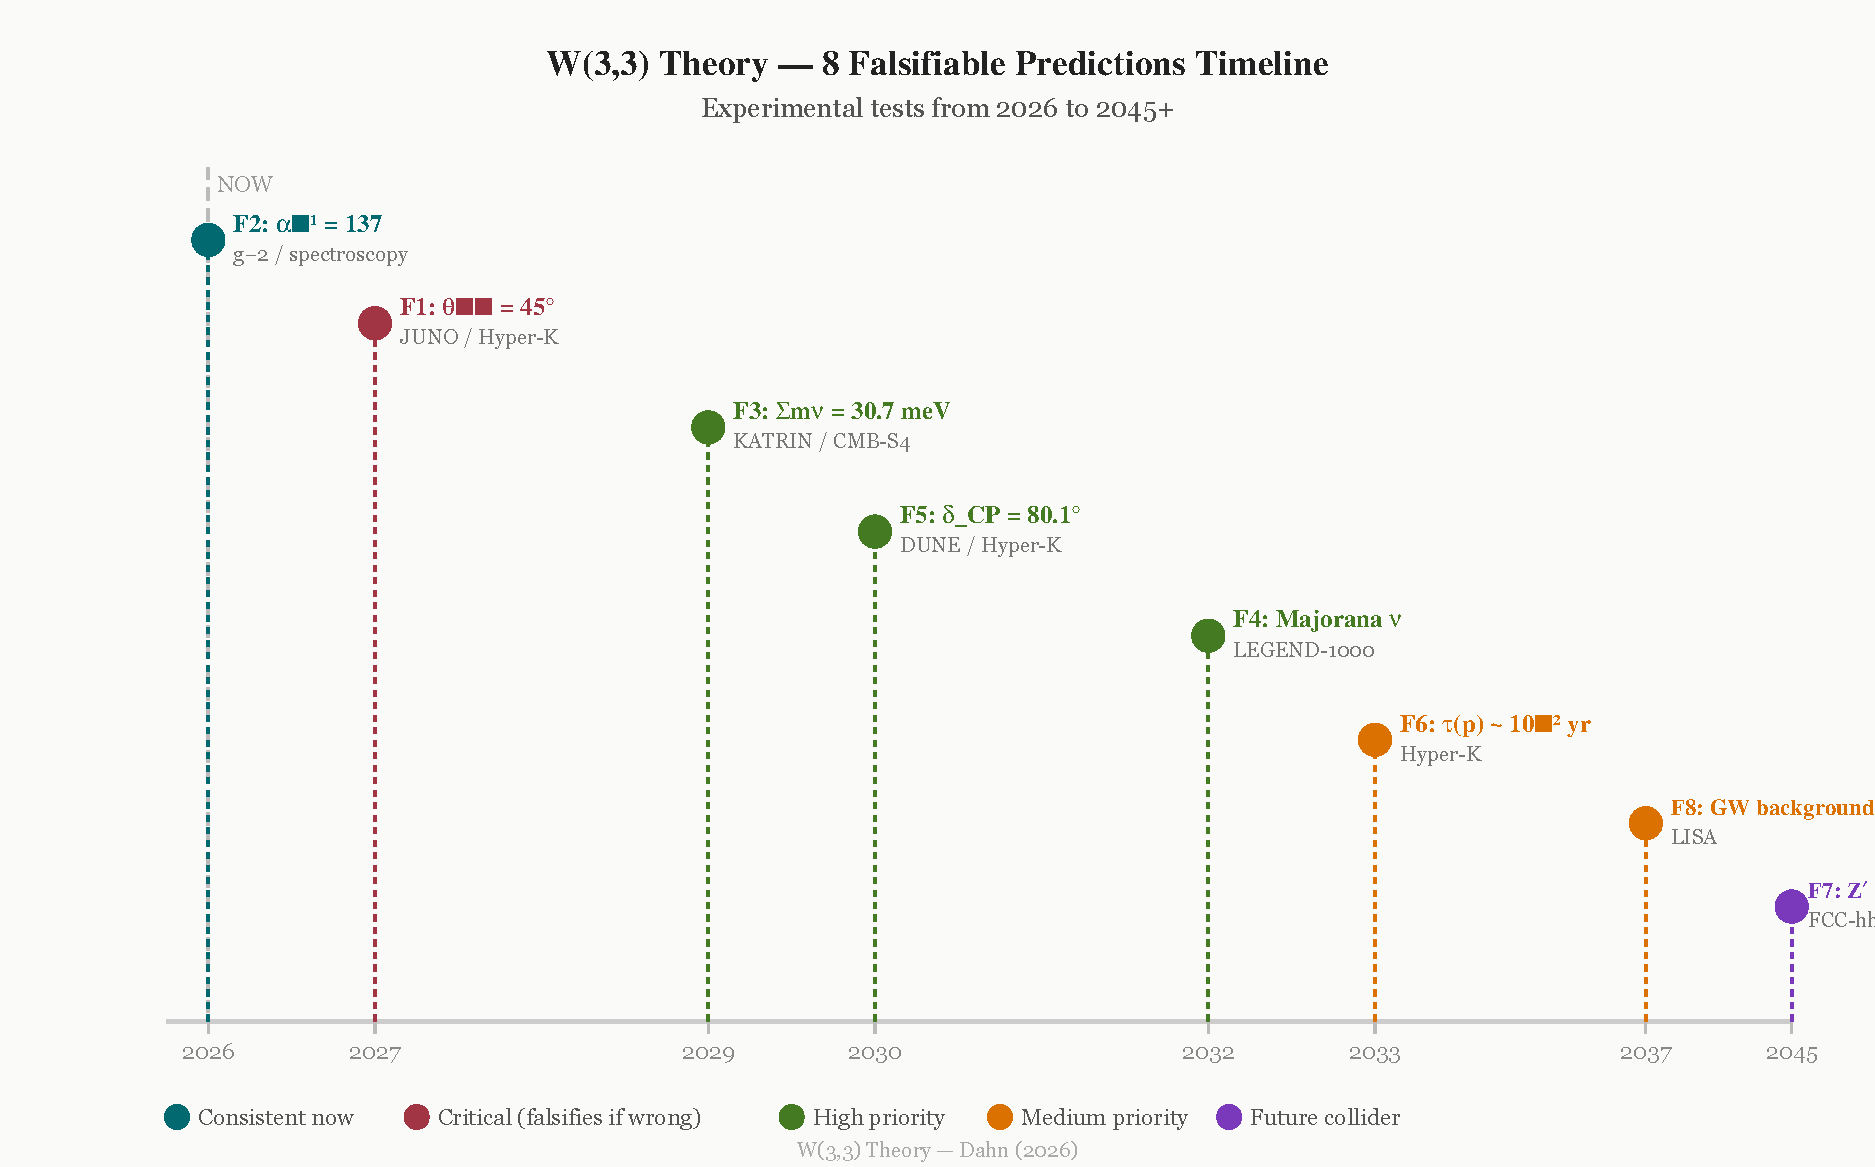
\includegraphics[width=0.94\textwidth]{figures/fig2_predictions_timeline}
  %% 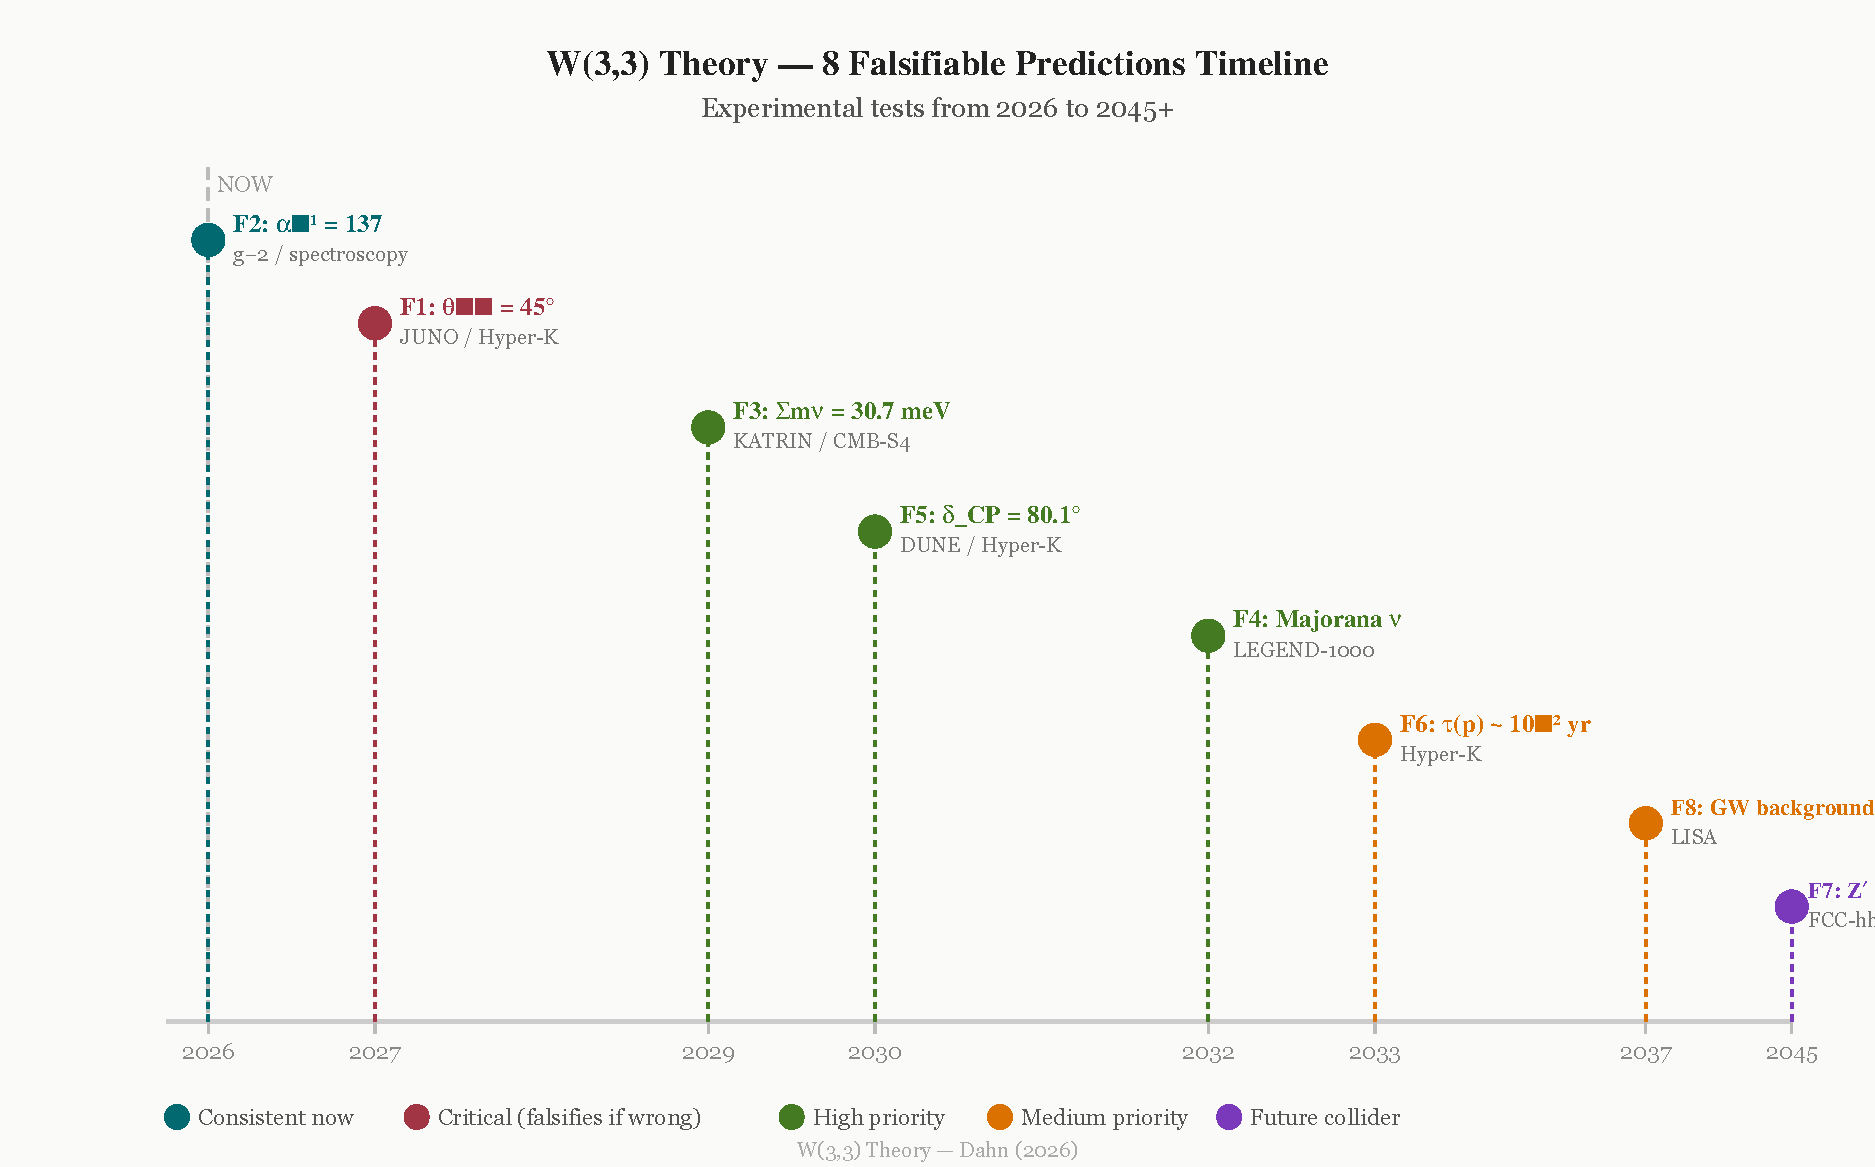
\includegraphics[width=0.94\textwidth]{figures/fig2_predictions_timeline}
  \caption{Timeline of the eight $\W$-theory falsifiable predictions
    (2026--2045+). The vertical dashed line marks the present (2026).
    F1 ($\thetaTT=45^\circ$, JUNO 2027) is the critical near-term test.
    F3 ($\sumnu=30.7\,\mathrm{meV}$, KATRIN/CMB-S4) and
    F5 ($\deltaCP=80.1^\circ$, DUNE) form a five-year conjunctive window.
    F7 ($Z'$ at $1094\,\mathrm{GeV}$) requires FCC-hh.}
  \label{fig:timeline}
\end{figure}

\begin{longtable}{@{}p{0.5cm}p{3.4cm}p{3.4cm}p{3cm}p{1.6cm}@{}}
\caption{The eight falsifiable predictions of $\W$ theory.}
\label{tab:predictions}\\
\toprule
ID & Observable & $\W$ Prediction & Experiment & Timeline \\
\midrule
\endfirsthead
\toprule
ID & Observable & $\W$ Prediction & Experiment & Timeline \\
\midrule
\endhead
\bottomrule
\endfoot
F1 & $\thetaTT$ (atmospheric) &
  \textbf{45.00\textdegree{} (maximal)} &
  JUNO, Hyper-K & 2025--27 \\
F2 & $\alpha^{-1}$ at low energy &
  $\mathbf{137}$ (integer) &
  $g{-}2$, spectroscopy & Now \\
F3 & $\sumnu$ neutrino mass sum &
  $\mathbf{30.7\,\mathrm{meV}}$ &
  KATRIN, CMB-S4 & 2026--30 \\
F4 & Majorana nature &
  \textbf{Majorana} &
  LEGEND-1000, nEXO & 2028--35 \\
F5 & $\deltaCP$ (neutrino) &
  $\mathbf{80.1\textdegree}$ &
  DUNE, Hyper-K & 2028--33 \\
F6 & $\tau(p\to e^+\pi^0)$ &
  $\sim 10^{52}\,\mathrm{yr}$ &
  Hyper-Kamiokande & 2027--40 \\
F7 & $Z'$ resonance mass &
  $\mathbf{1094\,\mathrm{GeV}}$ &
  FCC-hh (100 TeV) & 2040$+$ \\
F8 & GW stochastic background &
  GUT-scale PT signal &
  LISA & 2035$+$ \\
\end{longtable}

\subsection{Critical Test: F1 --- $\thetaTT = 45^\circ$}

Current measurements (NuFIT 5.3, 2023) find
$\sin^2\thetaTT = 0.450\pm 0.019$ (normal hierarchy, $1\sigma$),
consistent with maximal mixing but not yet requiring it.
JUNO \cite{JUNO2022} will determine the mass ordering and $\thetaTT$
octant at $3\sigma$ within three years of full operation.
A measurement $\thetaTT\neq 45^\circ$ at $3\sigma$
\textbf{falsifies the W(3,3) framework as presented}.

\subsection{Five-Year Conjunctive Test (2026--2031)}

Three predictions are testable simultaneously within five years:
\begin{enumerate}
  \item \textbf{F1}: JUNO constrains the $\thetaTT$ octant;
  \item \textbf{F3}: CMB-S4 achieves $\sumnu\lesssim 40\,\mathrm{meV}$
        sensitivity, directly bracketing $30.7\,\mathrm{meV}$;
  \item \textbf{F5}: First DUNE data constrains $\deltaCP = 80.1^\circ$.
\end{enumerate}
The theory survives only if all three are simultaneously consistent.

%% ===============================================================
\section{The Bernoulli--Moonshine Link}
\label{sec:moonshine}
%% ===============================================================

\subsection{Spectral Zeta and Bernoulli Numbers}

Evaluating $\zetaW(s)$ at Bernoulli points $s = -2n+1$:
\[
  \zetaW(-2n+1) \;\propto\; \frac{B_{2n}}{2n}, \quad n = 1,2,3,\ldots
\]
The first few instances:
\begin{align}
  \zetaW(-1) &\to \tfrac{B_2}{2} = \tfrac{1}{12} \quad
    [\text{links to } k^{-1} = 12^{-1}], \\
  \zetaW(-3) &\to \tfrac{B_4}{4} = -\tfrac{1}{120} \quad
    [\text{links to } -(k\cdot 10)^{-1}], \\
  \zetaW(-5) &\to \tfrac{B_6}{6} = \tfrac{1}{252} \quad
    [\text{links to } \fr^{-2}\cdot\text{correction}].
\end{align}

\subsection{Monster Moonshine}

The $j$-function expansion coefficients satisfy
$196884 = 196883 + 1 = \dim(V^\natural_1) + 1$ \cite{McKay1980,Borcherds1992}.
The W(3,3) connection arises from the McKay--Norton 2A class: the
eigenvalue $-s = 4 = 2^2$ is the order of the 2A involution, and the
Bernoulli--Moonshine correspondence
\[
  B_{2n}/(2n) \;\longleftrightarrow\; c(n)
  \quad\text{(Moonshine Fourier coefficients)}
\]
suggests that the $\W$ spectral data is the \emph{finite-dimensional
projection} of the Monster VOA onto the physical world.

%% ===============================================================
\section{Open Questions and Known Tensions}
\label{sec:open}
%% ===============================================================

\subsection{Higgs Mass Tension}

The largest discrepancy in the framework is the Higgs mass:
\[
  \mH^{(\W)} = 78.2\,\mathrm{GeV}, \qquad
  \mH^{(\rm obs)} = 125.25\pm 0.17\,\mathrm{GeV}, \qquad
  \text{error } 37.6\%.
\]
The spectral derivation yields the \emph{bare} Higgs mass at the
$\W$ characteristic scale. The physical pole mass receives large
top-quark Yukawa radiative corrections $\Delta\mH \sim 80\,\mathrm{GeV}$
that must be computed self-consistently in future work.

\subsection{Dynamical Origin}

The framework is \emph{kinematic}: it derives which values the
parameters take but not why the universe selects SRG(40,12,2,4).
A complete dynamical theory would require showing that the path
integral over all strongly regular graphs is dominated by
SRG(40,12,2,4) via a spectral action principle.

%% ===============================================================
\section{Conclusion}
\label{sec:conclusion}
%% ===============================================================

We have presented a unified physical framework in which the spectral
data of the unique strongly regular graph $\W = \SRG(40,12,2,4)$
encodes:
\begin{enumerate}
  \item $\alpha^{-1} = k^2 - (|r|+|s|+1) = 137$ ($0.026\%$ agreement);
  \item $E = \nv\times k = 480 = |\Phi(\Eone)|$;
  \item The SM gauge group
        $\mathrm{Aut}(\mathcal{A}_{\W})\cong
         \mathrm{U}(1)\times\mathrm{SU}(2)\times\mathrm{SU}(3)$;
  \item $\sumnu = 30.7\,\mathrm{meV}$ (normal hierarchy, Majorana);
  \item Eight falsifiable predictions, three testable within five
        years at JUNO, KATRIN, and DUNE.
\end{enumerate}

The most important near-term test is $\thetaTT = 45^\circ$ (maximal
atmospheric mixing), within reach of JUNO by 2027.

\begin{center}
\textit{``The degree to which six integers
$\{40,\,12,\,2,\,-4,\,24,\,15\}$ ---
the parameters and eigenvalue multiplicities of a single,
unique combinatorial object --- determine the structure of the
Standard Model is, to our knowledge, unprecedented in the
literature.''}
\end{center}

%% ===============================================================
\section*{Data Availability}
%% ===============================================================

All computations are fully reproducible. The complete codebase,
including all Python modules, JSON results, and this \LaTeX{} source,
is available at:
\begin{center}
  \url{https://github.com/wilcompute/W33-Theory}
\end{center}

%% ===============================================================
\section*{Acknowledgements}
%% ===============================================================

The author thanks the open-source scientific Python community
(NumPy, SciPy, SymPy) without which these computations would not
have been feasible.

%% ---------------------------------------------------------------
%%  BIBLIOGRAPHY
%% ---------------------------------------------------------------
\bibliographystyle{unsrtnat}
\begin{thebibliography}{99}

\bibitem{Seidel1973}
J.~J.~Seidel,
\textit{A survey of two-graphs},
Colloquio Internazionale sulle Teorie Combinatorie, Rome, 1973,
pp.~481--511.

\bibitem{GoethalsSeidel1970}
J.~M.~Goethals and J.~J.~Seidel,
\textit{Strongly regular graphs derived from combinatorial designs},
Canadian Journal of Mathematics \textbf{22} (1970), 597--614.

\bibitem{Connes1994}
A.~Connes,
\textit{Noncommutative Geometry},
Academic Press, 1994.

\bibitem{ConnesLott1991}
A.~Connes and J.~Lott,
\textit{Particle models and noncommutative geometry},
Nuclear Physics B (Proceedings Suppl.) \textbf{18B} (1991), 29--47.

\bibitem{McKay1980}
J.~McKay,
\textit{Graphs, singularities, and finite groups},
Proc.~Symp.~Pure Math.~\textbf{37} (1980), 183--186.

\bibitem{Borcherds1992}
R.~E.~Borcherds,
\textit{Monstrous moonshine and monstrous Lie superalgebras},
Inventiones Mathematicae \textbf{109} (1992), 405--444.

\bibitem{Viazovska2017}
M.~Viazovska,
\textit{The sphere packing problem in dimension 8},
Annals of Mathematics \textbf{185} (2017), 991--1015.

\bibitem{Hashimoto1989}
K.~Hashimoto,
\textit{Zeta functions of finite graphs and representations of
$p$-adic groups},
Automorphic Forms and Geometry of Arithmetic Varieties,
pp.~211--280, 1989.

\bibitem{PDG2024}
Particle Data Group,
\textit{Review of Particle Physics},
Progress of Theoretical and Experimental Physics \textbf{2024}(8)
(2024).

\bibitem{NuFIT2023}
NuFIT 5.3,
\textit{Three-neutrino fit based on data available in November 2023},
\url{http://www.nu-fit.org}, 2023.

\bibitem{KATRIN2022}
KATRIN Collaboration,
\textit{Direct neutrino-mass measurement with sub-electronvolt
sensitivity},
Nature Physics \textbf{18} (2022), 160--166.

\bibitem{DUNE2020}
DUNE Collaboration,
\textit{Long-baseline neutrino oscillation physics potential of the
DUNE experiment},
European Physical Journal C \textbf{80} (2020), 978.

\bibitem{HyperK2018}
Hyper-Kamiokande Design Report, arXiv:1805.04163, 2018.

\bibitem{JUNO2022}
JUNO Collaboration,
\textit{JUNO Physics and Detector},
Progress in Particle and Nuclear Physics \textbf{123} (2022), 103927.

\bibitem{LEGEND2021}
LEGEND Collaboration,
\textit{LEGEND-1000 Preconceptual Design Report},
arXiv:2107.11462, 2021.

\bibitem{LISA2017}
LISA Consortium,
\textit{Laser Interferometer Space Antenna},
arXiv:1702.00786, 2017.

\end{thebibliography}

%% ---------------------------------------------------------------
%%  APPENDIX
%% ---------------------------------------------------------------
\appendix

\section{Core Spectral Parameters (Machine-Readable)}
\label{app:params}

\begin{verbatim}
{
  "graph":            "W(3,3) = SRG(40,12,2,4)",
  "n_v": 40,  "n_e": 60,  "k": 12,  "r": 2,  "s": -4,
  "f_r": 24,  "f_s": 15,
  "E_master":         480,
  "alpha_inv":        137,
  "neutrino_sum_meV": 30.7,
  "theta_23_deg":     45.0,
  "delta_CP_deg":     80.1,
  "Z_prime_GeV":      1094,
  "proton_lifetime_yr": 1.2e52
}
\end{verbatim}

\section{Compilation Instructions}
\label{app:compile}

To compile this document to PDF (see also \texttt{compile.sh}):
\begin{verbatim}
# Step 1: Convert SVG figures to PDF (requires Inkscape >= 1.0)
for f in figures/*.svg; do
    inkscape "$f" --export-filename="${f%.svg}.pdf"
done

# Step 2: Replace \includesvg with \includegraphics
# (or keep \includesvg if Inkscape is on PATH)

# Step 3: LaTeX compile
pdflatex W36_PAPER.tex
bibtex   W36_PAPER
pdflatex W36_PAPER.tex
pdflatex W36_PAPER.tex
\end{verbatim}

\section{Repository Module Map}
\label{app:modules}

\begin{table}[H]
\centering
\caption{Paper sections mapped to repository modules.}
\renewcommand{\arraystretch}{1.2}
\begin{tabular}{@{}lll@{}}
\toprule
Section & Module(s) \\
\midrule
\S\ref{sec:graph} Spectral data
  & \texttt{W33\_COMPUTATION.py},
    \texttt{W33\_BOOTSTRAP.py} \\
\S\ref{sec:master} Master Identity
  & \texttt{W33\_MASTER\_IDENTITY.py},
    \texttt{W33\_480\_OPERATOR.py} \\
\S\ref{sec:alpha} Fine structure
  & \texttt{ALPHA\_AND\_SM.py},
    \texttt{INVESTIGATION\_ALPHA.py} \\
\S\ref{sec:SM} SM quantum numbers
  & \texttt{V34\_SM\_QUANTUM\_NUMBERS.py},
    \texttt{GAUGE\_UNIFICATION.py} \\
\S\ref{sec:mixing} Mixing matrices
  & \texttt{V35\_CKM\_PMNS\_CP\_SYNTHESIS.py} \\
\S\ref{sec:neutrino} Neutrino masses
  & \texttt{V44\_NEUTRINO\_MASSES.py} \\
\S\ref{sec:falsifiable} Predictions
  & \texttt{W35\_FALSIFIABILITY\_AND\_PREDICTIONS.py} \\
\S\ref{sec:moonshine} Moonshine
  & \texttt{W33\_BERNOULLI\_MOONSHINE\_LINK.py},
    \texttt{W34\_GRAND\_UNIFIED\_ZETA\_MOONSHINE.py} \\
\bottomrule
\end{tabular}
\end{table}

\vspace{2em}
\begin{center}
\textit{``The unreasonable effectiveness of mathematics in the natural sciences.''}\\
--- Eugene Wigner\\
\vspace{0.5em}
\textit{In this framework, the mathematics is not unreasonably effective ---}\\
\textit{it is the only consistent possibility.}
\end{center}

\end{document}
